%% Calling C Code in Rust
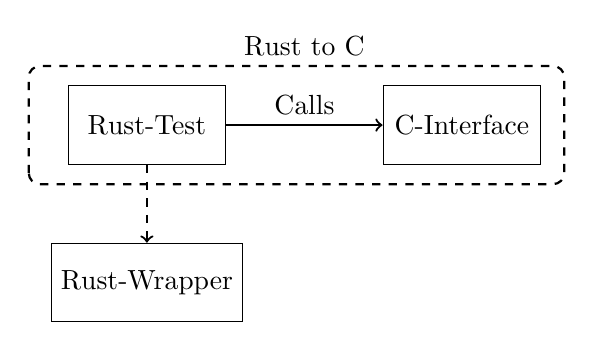
\begin{tikzpicture}asynchronous
  % Nodes
  \node (RS) [rectangle, draw, minimum height=1cm, minimum width=2cm] at (0, 0) {Rust-Test};
  \node (C) [rectangle, draw, minimum height=1cm, minimum width=2cm] at (4, 0) {C-Interface};
  \node (WRAP) [rectangle, draw, minimum height=1cm, minimum width=2cm] at (0, -2) {Rust-Wrapper};
  % Arrows
  \draw[->, thick] (RS) -- (C) node[midway, above] {Calls};
  \draw[->, dashed, thick] (RS) -- (WRAP) node[midway, above] {};
  % Header
  \node (title) at (2, 1) {Rust to C};
  % Dashed lines
  \draw[dashed, thick, rounded corners] (-1.5, -0.75) rectangle (5.3, 0.75);
\end{tikzpicture}

\hfill \break %% newline

%% RS can *use* C results
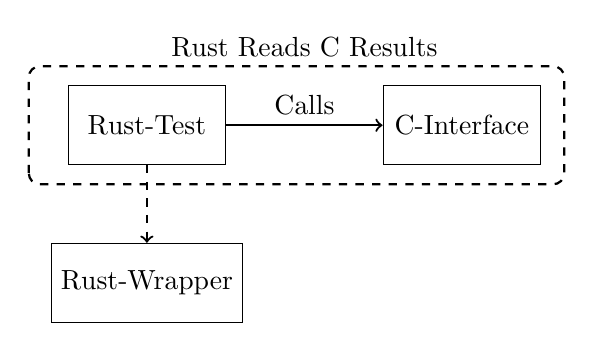
\begin{tikzpicture}asynchronous
  % Nodes
  \node (RS) [rectangle, draw, minimum height=1cm, minimum width=2cm] at (0, 0) {Rust-Test};
  \node (C) [rectangle, draw, minimum height=1cm, minimum width=2cm] at (4, 0) {C-Interface};
  \node (WRAP) [rectangle, draw, minimum height=1cm, minimum width=2cm] at (0, -2) {Rust-Wrapper};
  % Arrows
  \draw[->, thick] (RS) -- (C) node[midway, above] {Calls};
  \draw[->, dashed, thick] (RS) -- (WRAP) node[midway, above] {};
  % Header
  \node (title) at (2, 1) {Rust Reads C Results};
  % Dashed lines
  \draw[dashed, thick, rounded corners] (-1.5, -0.75) rectangle (5.3, 0.75);
\end{tikzpicture}

\hfill \break %% newline

%% Converting C types to Rust types
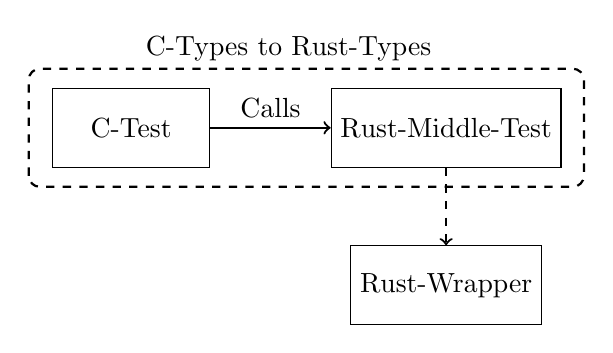
\begin{tikzpicture}asynchronous
  % Nodes
  \node (C) [rectangle, draw, minimum height=1cm, minimum width=2cm] at (0, 0) {C-Test};
  \node (RS-TEST) [rectangle, draw, minimum height=1cm, minimum width=2cm] at (4, 0) {Rust-Middle-Test};
  \node (RS) [rectangle, draw, minimum height=1cm, minimum width=2cm] at (4, -2) {Rust-Wrapper};
  % Arrows
  \draw[->, thick] (C) -- (RS-TEST) node[midway, above] {Calls};
  \draw[->, dashed, thick] (RS-TEST) -- (RS) node[midway, above] {};
  % Header
  \node (title) at (2, 1) {C-Types to Rust-Types};
  % Dashed lines
  \draw[dashed, thick, rounded corners] (-1.3, -0.75) rectangle (5.75, 0.75);
\end{tikzpicture}

\hfill \break %% newline

%% Calling Rust Plugins
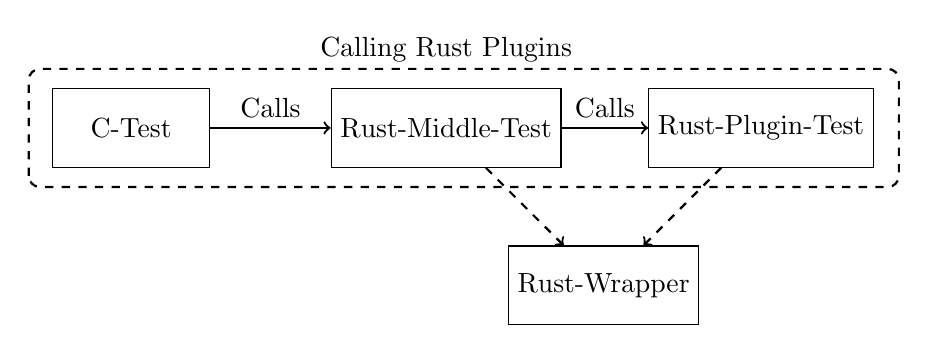
\begin{tikzpicture}asynchronous
  % Nodes
  \node (C) [rectangle, draw, minimum height=1cm, minimum width=2cm] at (0, 0) {C-Test};
  \node (RS-TEST) [rectangle, draw, minimum height=1cm, minimum width=2cm] at (4, 0) {Rust-Middle-Test};
  \node (RS) [rectangle, draw, minimum height=1cm, minimum width=2cm] at (6, -2) {Rust-Wrapper};
  \node (P) [rectangle, draw, minimum height=1cm, minimum width=2cm] at (8, 0) {Rust-Plugin-Test};
  % Arrows
  \draw[->, thick] (C) -- (RS-TEST) node[midway, above] {Calls};
  \draw[->, dashed, thick] (RS-TEST) -- (RS) node[midway, above] {};
  \draw[->, dashed, thick] (P) -- (RS) node[midway, above] {};
  \draw[->, thick] (RS-TEST) -- (P) node[midway, above] {Calls};
  % Header
  \node (title) at (4, 1) {Calling Rust Plugins};
  % Dashed lines
  \draw[dashed, thick, rounded corners] (-1.3, -0.75) rectangle (9.75, 0.75);
\end{tikzpicture}

\hfill \break %% newline

%% Calling * Plugins
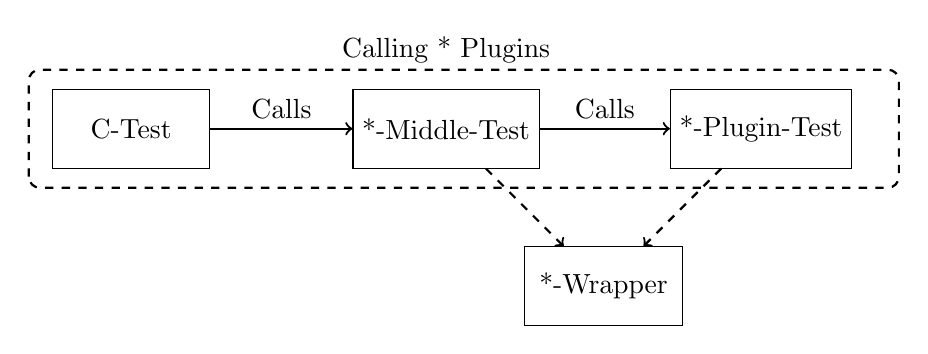
\begin{tikzpicture}asynchronous
  % Nodes
  \node (C) [rectangle, draw, minimum height=1cm, minimum width=2cm] at (0, 0) {C-Test};
  \node (-TEST) [rectangle, draw, minimum height=1cm, minimum width=2cm] at (4, 0) {*-Middle-Test};
  \node (W) [rectangle, draw, minimum height=1cm, minimum width=2cm] at (6, -2) {*-Wrapper};
  \node (P) [rectangle, draw, minimum height=1cm, minimum width=2cm] at (8, 0) {*-Plugin-Test};
  % Arrows
  \draw[->, thick] (C) -- (-TEST) node[midway, above] {Calls};
  \draw[->, dashed, thick] (-TEST) -- (W) node[midway, above] {};
  \draw[->, dashed, thick] (P) -- (W) node[midway, above] {};
  \draw[->, thick] (-TEST) -- (P) node[midway, above] {Calls};
  % Header
  \node (title) at (4, 1) {Calling * Plugins};
  % Dashed lines
  \draw[dashed, thick, rounded corners] (-1.3, -0.75) rectangle (9.75, 0.75);
\end{tikzpicture}


